\begin{problem}{Counting Stairs}{standard input}{standard output}{3 seconds}{512 megabytes}

Remember Barney from problem B? Barney's older sister Cecilia often watches him play with his set of cubes. She also joins Barney in his games and prevails most of the time, shaking his confidence on a daily basis.

One day Cecilia noticed Barney struggling to build a \textit{symmetric stair} with his $n$ cubes. She immediately told him she could not just build a symmetric stair, but even calculate the number of different symmetric stairs consisting of $n$ cubes! Can you?

Recall that a \textit{symmetric stair} consists of one or more towers of cubes, where the heights of towers are \textit{non-increasing} from left to right, and is symmetric with respect to the $x = y$ line (where the $x$-axis is horizontal and oriented to the right, and the $y$-axis is vertical and oriented upwards). For a more detailed explanation, please refer to problem B statement.

The number of different symmetric stairs can be quite large, so you need to calculate it modulo $998\,244\,353$.

\InputFile
The input contains multiple test cases.

The first line of the input contains a single integer $t$~--- the number of test cases ($1 \le t \le 10^4$). Each of the following $t$ lines contains a single integer $n_i$~--- the number of cubes in the $i$-th test case ($1 \le n_i \le 2 \cdot 10^5$).

\OutputFile
For each test case, output a line with a single integer~--- the number of symmetric stairs with exactly $n_i$ cubes, modulo $998\,244\,353$.

\Example

\begin{example}
\exmp{4
3
5
17
25
}{1
1
5
12
}%
\end{example}

\Note
All different symmetric stairs with $n = 17$ cubes are shown below:

\begin{center}
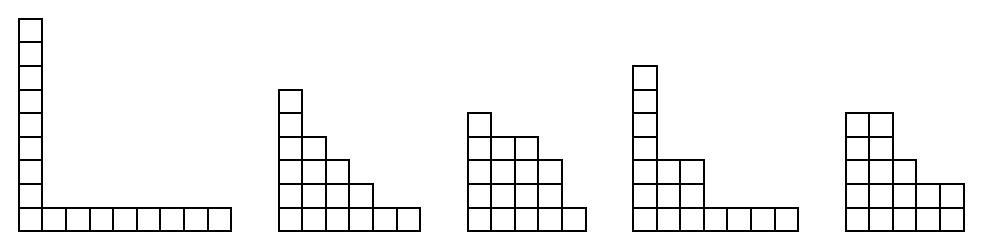
\includegraphics{sample-1.eps}
\end{center}


\end{problem}

